\section{Polynomial Interpolator Class}

\subsection{Methods}

\begin{itemize}
	\item \uline{Initialization:} Requires reference element/GeometryType, interpolatory vertex vector and interpolation order
	\item \uline{dofPerOrder:} Number of interpolatory vertices required for a given element type, dimension and interpolation order. For a simplex this quantity is
	\[ {DoF}_{dim}^{ord} = \{ \{ 2,3,4,5,6 \}, \{ 3,6,10,15,21 \}, \{ 4,10,20,35,56 \} \} \]
	\item \uline{cornerID:} The id number of a corner in the interpolatory vertex vector. For the simplices is calculated as follows:
		\subitem -for edge $\{ 0, \; ord \}$
		\subitem -for triangle $\{0, \; ord, \; {DoF}_{dim}^{ord} - 1\}$
		\subitem -for tetrahedron $\{0, \; ord, \; ord (ord + 3) / 2, \; {DoF}_{dim}^{ord} - 1\}$
	\item \uline{simplexGrid:} These 3 methods implement the functionality discussed in section \ref{subsection-simplexgrid}. They return a vector of indices which the grid points take in the d-dimensional matrix, and that vector divided by the interpolation order, which is exactly the local coordinates of the reference simplex grid.
	\item \uline{lagrangePolynomial:} Evaluates the i-th Lagrange Polynomial $L_i(\vec{r})$ for a given $i$ and a given local coordinate. Lagrange polynomials in this case are given explicitly for all orders to accellerate computation.
	\item \uline{realCoordinate:} Evaluates the global coordinate given a local coordinate. Computes the scalar product $\vec{p}(\vec{r}) = \sum_i \vec{p}_i L_i (\vec{r})$.
	\item \uline{interpolatoryVectorAnalytical:} Produces an analytical map from local to global coordinates in terms of polynomial vector.
		\subitem 0) Constructs local grid points $\vec{r}_i$ as given in \ref{subsection-simplexgrid}.		
		\subitem 1) Constructs monomial basis $\vec{z}^{ord}(\vec{r})$ as given in the beginning of section \ref{section-interppoly}
		\subitem 2) Evaluates all monomials $\vec{z}^{ord}(\vec{r})$ at all local grid points $\vec{r}_i$, assembling the DynamicMatrix V
		\subitem 3) Computes all lagrange polynomials using $\vec{L}(\vec{r}) = V^{-1} \vec{z}^{ord}(\vec{r})$
		\subitem 4) Computes the analytical map $\vec{p}(\vec{r}) = \sum_i \vec{p}_i L_i (\vec{r})$.
	\item \uline{SubentityInterpolators} Constructs Interpolator classes for each $\dim - 1$ subentity of the given element. Only allowed for elements of dimensions 2 and 3.
		\subitem - At the moment a rather crude algorithm is employed. To find the vertices corresponding to a given boundary, the order numbers of simplexGrid are written in a $(ord + 1) \times (ord + 1) \times (ord + 1)$ matrix, which is then used to easier locate the indices of the boundary interpolatory points in the vertex vector.
		\subitem - Certain orientation convention is chosen for the provided sub-entitiy interpolators, to simplify the future calculation of the outwards normals. The convention for edge orientations for a triangle $(012)$ are $(01)$, $(12)$ and $(20)$. The convention for triangle orientations for a tetrahedron $(0123)$ are $(012)$, $(023)$, $(213)$ and $(031)$.
\end{itemize}

\begin{figure}[hp]
    \centering
    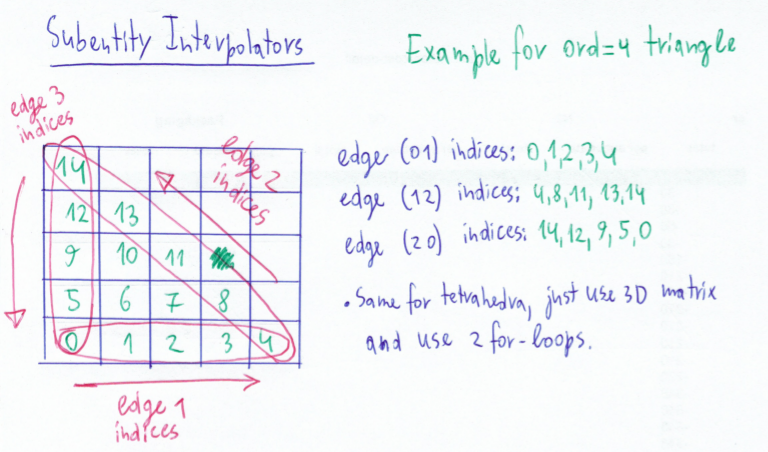
\includegraphics[scale=0.5]{doc-pics/pic-subentity-interpolators-method.png}
    %\caption{Awesome Image}
    %\label{fig:awesome_image}
\end{figure}


\subsection{Tests}

\noindent
For each dimension several linear and polynomial Functors are defined which act as pre-defined local-to-global maps. Then, for a simplex of each dimension there is a testing routine which is run for every applicable Functor. The tests are as follows:
\begin{itemize}
	\item For each order generate a local grid and sample the given functor to obtain global coordinates for interpolation points and thus construct the interpolator.
	\item First test requests a global coordinate for each local grid point, both using explicit function $realCoordinate$ and by evaluating the analytical polynomial provided by $interpolatoryVectorAnalytical$. Then the 3 results are compared. For this test, all 3 results must match independent of Functor and interpolation order.
	\item Second test requests a global coordinate for a random set of local coordinates, also comparing the correct result with explicit and analytical functionality. Explicit and analytical results should be equal to each other for any test since they do the same thing. However, they will match to the true result only if the polynomial order of the Functor is lower or equal to the one being tested, and most likely should fail for lower orders.
\end{itemize}

\textbf{TODO:}
\begin{itemize}
	\item The tests must be automatized such that the program throws an error if a test fails.
	\item Would be useful to test the method $SubentityInterpolators$ which is not tested at the moment, but is indirectly tested later in the LagrangeGeometry tests.
\end{itemize}